% Created by tikzDevice version 0.12.6 on 2026-08-11 03:14:43
% !TEX encoding = UTF-8 Unicode
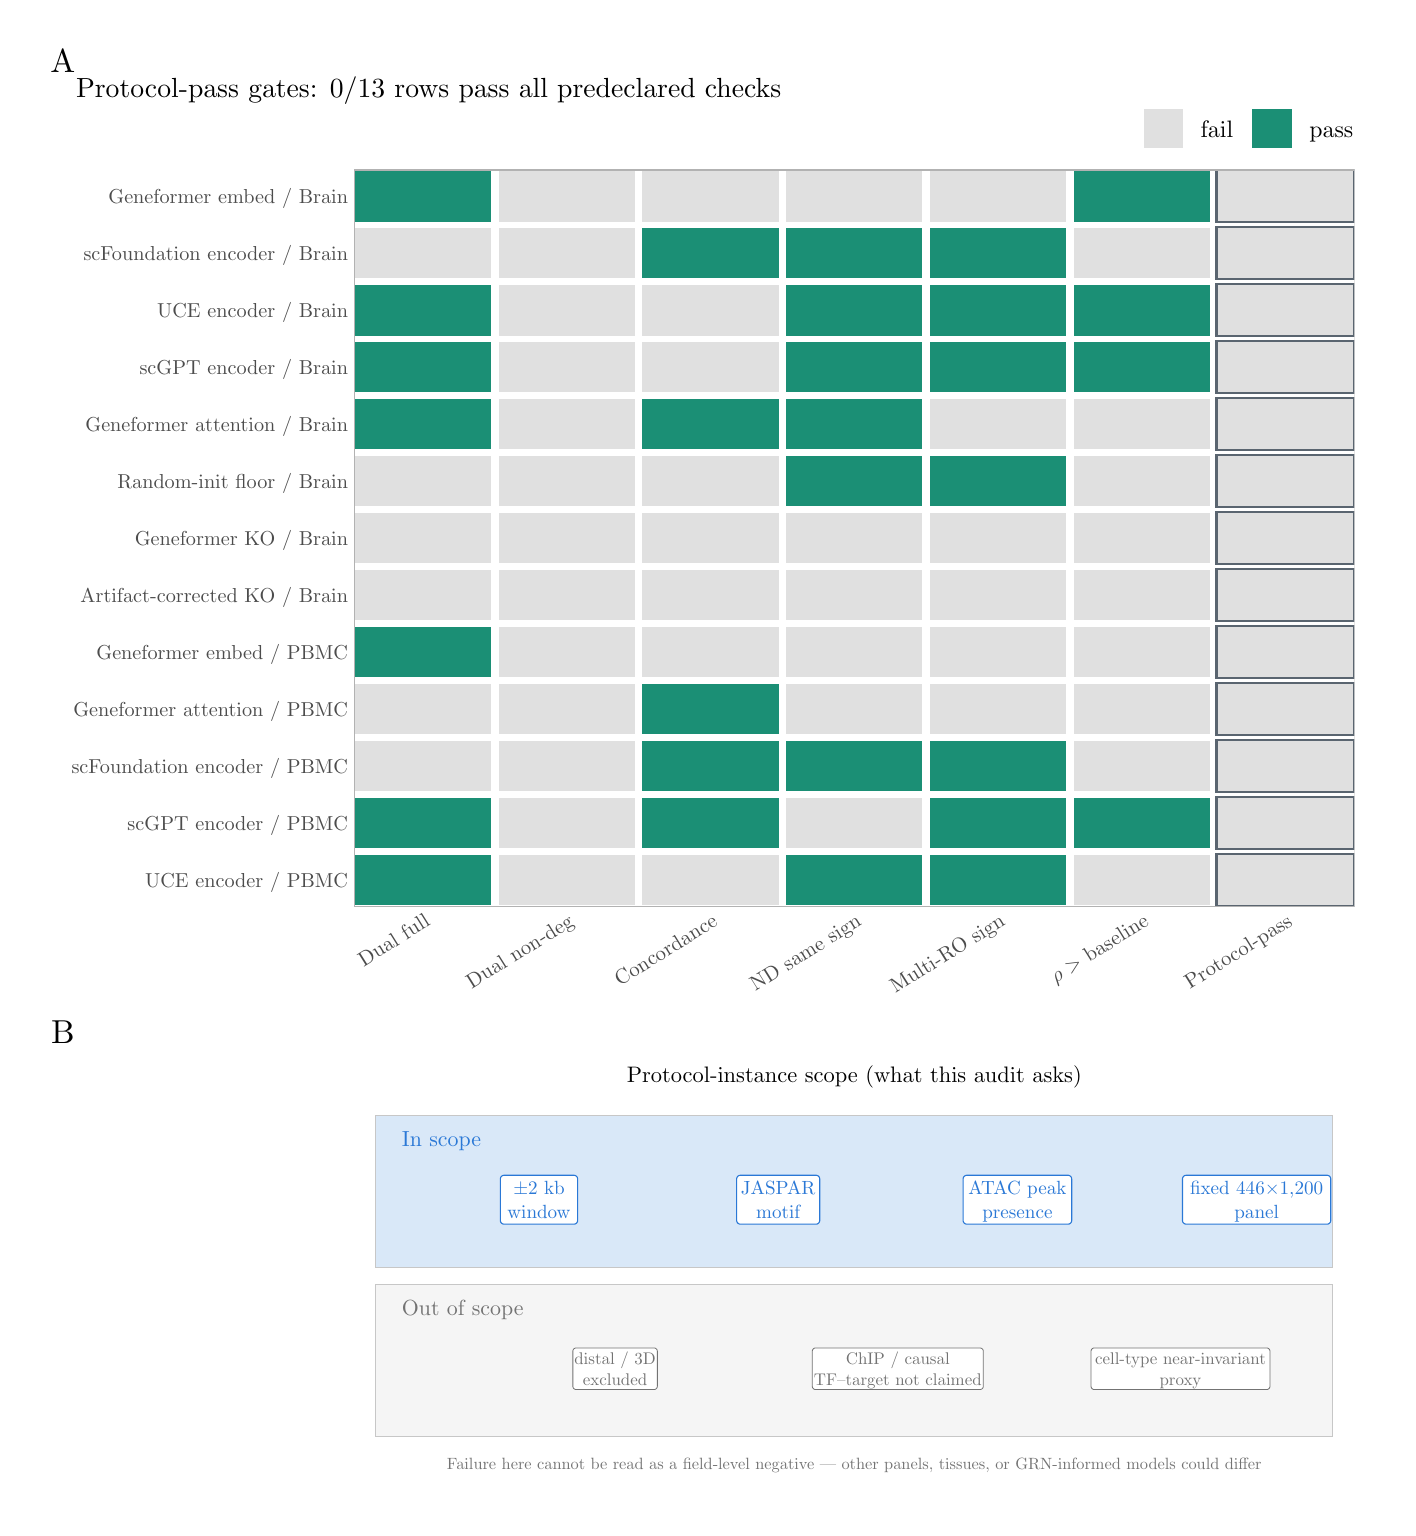
\begin{tikzpicture}[x=1pt,y=1pt]
\definecolor{fillColor}{RGB}{255,255,255}
\path[use as bounding box,fill=fillColor,fill opacity=0.00] (0,0) rectangle (491.44,534.80);
\begin{scope}
\path[clip] (  0.00,  0.00) rectangle (491.44,534.80);
\definecolor{drawColor}{RGB}{255,255,255}
\definecolor{fillColor}{RGB}{255,255,255}

\path[draw=drawColor,line width= 0.6pt,line join=round,line cap=round,fill=fillColor] ( -0.00,  0.00) rectangle (491.44,534.80);
\end{scope}
\begin{scope}
\path[clip] (  4.00,181.98) rectangle (485.44,530.80);
\definecolor{drawColor}{RGB}{255,255,255}
\definecolor{fillColor}{RGB}{255,255,255}

\path[draw=drawColor,line width= 0.6pt,line join=round,line cap=round,fill=fillColor] (  4.00,181.98) rectangle (485.44,530.80);
\end{scope}
\begin{scope}
\path[clip] (  4.00,  3.00) rectangle (485.44,181.98);

\path[] (  4.00,  3.00) rectangle (485.44,181.98);
\end{scope}
\begin{scope}
\path[clip] (117.97,217.33) rectangle (479.44,483.40);
\definecolor{fillColor}{RGB}{255,255,255}

\path[fill=fillColor] (117.97,217.33) rectangle (479.44,483.40);
\definecolor{drawColor}{RGB}{255,255,255}
\definecolor{fillColor}{RGB}{27,143,117}

\path[draw=drawColor,line width= 0.6pt,fill=fillColor] (117.97,464.45) rectangle (167.83,483.40);
\definecolor{fillColor}{gray}{0.88}

\path[draw=drawColor,line width= 0.6pt,fill=fillColor] (117.97,443.86) rectangle (167.83,462.80);
\definecolor{fillColor}{RGB}{27,143,117}

\path[draw=drawColor,line width= 0.6pt,fill=fillColor] (117.97,423.26) rectangle (167.83,442.21);

\path[draw=drawColor,line width= 0.6pt,fill=fillColor] (117.97,402.67) rectangle (167.83,421.62);

\path[draw=drawColor,line width= 0.6pt,fill=fillColor] (117.97,382.08) rectangle (167.83,401.02);
\definecolor{fillColor}{gray}{0.88}

\path[draw=drawColor,line width= 0.6pt,fill=fillColor] (117.97,361.48) rectangle (167.83,380.43);

\path[draw=drawColor,line width= 0.6pt,fill=fillColor] (117.97,340.89) rectangle (167.83,359.84);

\path[draw=drawColor,line width= 0.6pt,fill=fillColor] (117.97,320.29) rectangle (167.83,339.24);
\definecolor{fillColor}{RGB}{27,143,117}

\path[draw=drawColor,line width= 0.6pt,fill=fillColor] (117.97,299.70) rectangle (167.83,318.65);
\definecolor{fillColor}{gray}{0.88}

\path[draw=drawColor,line width= 0.6pt,fill=fillColor] (117.97,279.11) rectangle (167.83,298.05);

\path[draw=drawColor,line width= 0.6pt,fill=fillColor] (117.97,258.51) rectangle (167.83,277.46);
\definecolor{fillColor}{RGB}{27,143,117}

\path[draw=drawColor,line width= 0.6pt,fill=fillColor] (117.97,237.92) rectangle (167.83,256.87);

\path[draw=drawColor,line width= 0.6pt,fill=fillColor] (117.97,217.33) rectangle (167.83,236.27);
\definecolor{fillColor}{gray}{0.88}

\path[draw=drawColor,line width= 0.6pt,fill=fillColor] (169.90,464.45) rectangle (219.76,483.40);

\path[draw=drawColor,line width= 0.6pt,fill=fillColor] (169.90,443.86) rectangle (219.76,462.80);

\path[draw=drawColor,line width= 0.6pt,fill=fillColor] (169.90,423.26) rectangle (219.76,442.21);

\path[draw=drawColor,line width= 0.6pt,fill=fillColor] (169.90,402.67) rectangle (219.76,421.62);

\path[draw=drawColor,line width= 0.6pt,fill=fillColor] (169.90,382.08) rectangle (219.76,401.02);

\path[draw=drawColor,line width= 0.6pt,fill=fillColor] (169.90,361.48) rectangle (219.76,380.43);

\path[draw=drawColor,line width= 0.6pt,fill=fillColor] (169.90,340.89) rectangle (219.76,359.84);

\path[draw=drawColor,line width= 0.6pt,fill=fillColor] (169.90,320.29) rectangle (219.76,339.24);

\path[draw=drawColor,line width= 0.6pt,fill=fillColor] (169.90,299.70) rectangle (219.76,318.65);

\path[draw=drawColor,line width= 0.6pt,fill=fillColor] (169.90,279.11) rectangle (219.76,298.05);

\path[draw=drawColor,line width= 0.6pt,fill=fillColor] (169.90,258.51) rectangle (219.76,277.46);

\path[draw=drawColor,line width= 0.6pt,fill=fillColor] (169.90,237.92) rectangle (219.76,256.87);

\path[draw=drawColor,line width= 0.6pt,fill=fillColor] (169.90,217.33) rectangle (219.76,236.27);

\path[draw=drawColor,line width= 0.6pt,fill=fillColor] (221.84,464.45) rectangle (271.70,483.40);
\definecolor{fillColor}{RGB}{27,143,117}

\path[draw=drawColor,line width= 0.6pt,fill=fillColor] (221.84,443.86) rectangle (271.70,462.80);
\definecolor{fillColor}{gray}{0.88}

\path[draw=drawColor,line width= 0.6pt,fill=fillColor] (221.84,423.26) rectangle (271.70,442.21);

\path[draw=drawColor,line width= 0.6pt,fill=fillColor] (221.84,402.67) rectangle (271.70,421.62);
\definecolor{fillColor}{RGB}{27,143,117}

\path[draw=drawColor,line width= 0.6pt,fill=fillColor] (221.84,382.08) rectangle (271.70,401.02);
\definecolor{fillColor}{gray}{0.88}

\path[draw=drawColor,line width= 0.6pt,fill=fillColor] (221.84,361.48) rectangle (271.70,380.43);

\path[draw=drawColor,line width= 0.6pt,fill=fillColor] (221.84,340.89) rectangle (271.70,359.84);

\path[draw=drawColor,line width= 0.6pt,fill=fillColor] (221.84,320.29) rectangle (271.70,339.24);

\path[draw=drawColor,line width= 0.6pt,fill=fillColor] (221.84,299.70) rectangle (271.70,318.65);
\definecolor{fillColor}{RGB}{27,143,117}

\path[draw=drawColor,line width= 0.6pt,fill=fillColor] (221.84,279.11) rectangle (271.70,298.05);

\path[draw=drawColor,line width= 0.6pt,fill=fillColor] (221.84,258.51) rectangle (271.70,277.46);

\path[draw=drawColor,line width= 0.6pt,fill=fillColor] (221.84,237.92) rectangle (271.70,256.87);
\definecolor{fillColor}{gray}{0.88}

\path[draw=drawColor,line width= 0.6pt,fill=fillColor] (221.84,217.33) rectangle (271.70,236.27);

\path[draw=drawColor,line width= 0.6pt,fill=fillColor] (273.77,464.45) rectangle (323.63,483.40);
\definecolor{fillColor}{RGB}{27,143,117}

\path[draw=drawColor,line width= 0.6pt,fill=fillColor] (273.77,443.86) rectangle (323.63,462.80);

\path[draw=drawColor,line width= 0.6pt,fill=fillColor] (273.77,423.26) rectangle (323.63,442.21);

\path[draw=drawColor,line width= 0.6pt,fill=fillColor] (273.77,402.67) rectangle (323.63,421.62);

\path[draw=drawColor,line width= 0.6pt,fill=fillColor] (273.77,382.08) rectangle (323.63,401.02);

\path[draw=drawColor,line width= 0.6pt,fill=fillColor] (273.77,361.48) rectangle (323.63,380.43);
\definecolor{fillColor}{gray}{0.88}

\path[draw=drawColor,line width= 0.6pt,fill=fillColor] (273.77,340.89) rectangle (323.63,359.84);

\path[draw=drawColor,line width= 0.6pt,fill=fillColor] (273.77,320.29) rectangle (323.63,339.24);

\path[draw=drawColor,line width= 0.6pt,fill=fillColor] (273.77,299.70) rectangle (323.63,318.65);

\path[draw=drawColor,line width= 0.6pt,fill=fillColor] (273.77,279.11) rectangle (323.63,298.05);
\definecolor{fillColor}{RGB}{27,143,117}

\path[draw=drawColor,line width= 0.6pt,fill=fillColor] (273.77,258.51) rectangle (323.63,277.46);
\definecolor{fillColor}{gray}{0.88}

\path[draw=drawColor,line width= 0.6pt,fill=fillColor] (273.77,237.92) rectangle (323.63,256.87);
\definecolor{fillColor}{RGB}{27,143,117}

\path[draw=drawColor,line width= 0.6pt,fill=fillColor] (273.77,217.33) rectangle (323.63,236.27);
\definecolor{fillColor}{gray}{0.88}

\path[draw=drawColor,line width= 0.6pt,fill=fillColor] (325.71,464.45) rectangle (375.57,483.40);
\definecolor{fillColor}{RGB}{27,143,117}

\path[draw=drawColor,line width= 0.6pt,fill=fillColor] (325.71,443.86) rectangle (375.57,462.80);

\path[draw=drawColor,line width= 0.6pt,fill=fillColor] (325.71,423.26) rectangle (375.57,442.21);

\path[draw=drawColor,line width= 0.6pt,fill=fillColor] (325.71,402.67) rectangle (375.57,421.62);
\definecolor{fillColor}{gray}{0.88}

\path[draw=drawColor,line width= 0.6pt,fill=fillColor] (325.71,382.08) rectangle (375.57,401.02);
\definecolor{fillColor}{RGB}{27,143,117}

\path[draw=drawColor,line width= 0.6pt,fill=fillColor] (325.71,361.48) rectangle (375.57,380.43);
\definecolor{fillColor}{gray}{0.88}

\path[draw=drawColor,line width= 0.6pt,fill=fillColor] (325.71,340.89) rectangle (375.57,359.84);

\path[draw=drawColor,line width= 0.6pt,fill=fillColor] (325.71,320.29) rectangle (375.57,339.24);

\path[draw=drawColor,line width= 0.6pt,fill=fillColor] (325.71,299.70) rectangle (375.57,318.65);

\path[draw=drawColor,line width= 0.6pt,fill=fillColor] (325.71,279.11) rectangle (375.57,298.05);
\definecolor{fillColor}{RGB}{27,143,117}

\path[draw=drawColor,line width= 0.6pt,fill=fillColor] (325.71,258.51) rectangle (375.57,277.46);

\path[draw=drawColor,line width= 0.6pt,fill=fillColor] (325.71,237.92) rectangle (375.57,256.87);

\path[draw=drawColor,line width= 0.6pt,fill=fillColor] (325.71,217.33) rectangle (375.57,236.27);

\path[draw=drawColor,line width= 0.6pt,fill=fillColor] (377.64,464.45) rectangle (427.50,483.40);
\definecolor{fillColor}{gray}{0.88}

\path[draw=drawColor,line width= 0.6pt,fill=fillColor] (377.64,443.86) rectangle (427.50,462.80);
\definecolor{fillColor}{RGB}{27,143,117}

\path[draw=drawColor,line width= 0.6pt,fill=fillColor] (377.64,423.26) rectangle (427.50,442.21);

\path[draw=drawColor,line width= 0.6pt,fill=fillColor] (377.64,402.67) rectangle (427.50,421.62);
\definecolor{fillColor}{gray}{0.88}

\path[draw=drawColor,line width= 0.6pt,fill=fillColor] (377.64,382.08) rectangle (427.50,401.02);

\path[draw=drawColor,line width= 0.6pt,fill=fillColor] (377.64,361.48) rectangle (427.50,380.43);

\path[draw=drawColor,line width= 0.6pt,fill=fillColor] (377.64,340.89) rectangle (427.50,359.84);

\path[draw=drawColor,line width= 0.6pt,fill=fillColor] (377.64,320.29) rectangle (427.50,339.24);

\path[draw=drawColor,line width= 0.6pt,fill=fillColor] (377.64,299.70) rectangle (427.50,318.65);

\path[draw=drawColor,line width= 0.6pt,fill=fillColor] (377.64,279.11) rectangle (427.50,298.05);

\path[draw=drawColor,line width= 0.6pt,fill=fillColor] (377.64,258.51) rectangle (427.50,277.46);
\definecolor{fillColor}{RGB}{27,143,117}

\path[draw=drawColor,line width= 0.6pt,fill=fillColor] (377.64,237.92) rectangle (427.50,256.87);
\definecolor{fillColor}{gray}{0.88}

\path[draw=drawColor,line width= 0.6pt,fill=fillColor] (377.64,217.33) rectangle (427.50,236.27);

\path[draw=drawColor,line width= 0.6pt,fill=fillColor] (429.58,464.45) rectangle (479.44,483.40);

\path[draw=drawColor,line width= 0.6pt,fill=fillColor] (429.58,443.86) rectangle (479.44,462.80);

\path[draw=drawColor,line width= 0.6pt,fill=fillColor] (429.58,423.26) rectangle (479.44,442.21);

\path[draw=drawColor,line width= 0.6pt,fill=fillColor] (429.58,402.67) rectangle (479.44,421.62);

\path[draw=drawColor,line width= 0.6pt,fill=fillColor] (429.58,382.08) rectangle (479.44,401.02);

\path[draw=drawColor,line width= 0.6pt,fill=fillColor] (429.58,361.48) rectangle (479.44,380.43);

\path[draw=drawColor,line width= 0.6pt,fill=fillColor] (429.58,340.89) rectangle (479.44,359.84);

\path[draw=drawColor,line width= 0.6pt,fill=fillColor] (429.58,320.29) rectangle (479.44,339.24);

\path[draw=drawColor,line width= 0.6pt,fill=fillColor] (429.58,299.70) rectangle (479.44,318.65);

\path[draw=drawColor,line width= 0.6pt,fill=fillColor] (429.58,279.11) rectangle (479.44,298.05);

\path[draw=drawColor,line width= 0.6pt,fill=fillColor] (429.58,258.51) rectangle (479.44,277.46);

\path[draw=drawColor,line width= 0.6pt,fill=fillColor] (429.58,237.92) rectangle (479.44,256.87);

\path[draw=drawColor,line width= 0.6pt,fill=fillColor] (429.58,217.33) rectangle (479.44,236.27);
\definecolor{drawColor}{RGB}{90,101,112}

\path[draw=drawColor,line width= 0.8pt] (429.58,464.45) rectangle (479.44,483.40);

\path[draw=drawColor,line width= 0.8pt] (429.58,443.86) rectangle (479.44,462.80);

\path[draw=drawColor,line width= 0.8pt] (429.58,423.26) rectangle (479.44,442.21);

\path[draw=drawColor,line width= 0.8pt] (429.58,402.67) rectangle (479.44,421.62);

\path[draw=drawColor,line width= 0.8pt] (429.58,382.08) rectangle (479.44,401.02);

\path[draw=drawColor,line width= 0.8pt] (429.58,361.48) rectangle (479.44,380.43);

\path[draw=drawColor,line width= 0.8pt] (429.58,340.89) rectangle (479.44,359.84);

\path[draw=drawColor,line width= 0.8pt] (429.58,320.29) rectangle (479.44,339.24);

\path[draw=drawColor,line width= 0.8pt] (429.58,299.70) rectangle (479.44,318.65);

\path[draw=drawColor,line width= 0.8pt] (429.58,279.11) rectangle (479.44,298.05);

\path[draw=drawColor,line width= 0.8pt] (429.58,258.51) rectangle (479.44,277.46);

\path[draw=drawColor,line width= 0.8pt] (429.58,237.92) rectangle (479.44,256.87);

\path[draw=drawColor,line width= 0.8pt] (429.58,217.33) rectangle (479.44,236.27);
\definecolor{drawColor}{gray}{0.70}

\path[draw=drawColor,line width= 0.5pt,line join=round,line cap=round] (117.97,217.33) rectangle (479.44,483.40);
\end{scope}
\begin{scope}
\path[clip] (  0.00,  0.00) rectangle (491.44,534.80);
\definecolor{drawColor}{gray}{0.30}

\node[text=drawColor,anchor=base east,inner sep=0pt, outer sep=0pt, scale=  0.73] at (115.77,224.11) {UCE encoder / PBMC};

\node[text=drawColor,anchor=base east,inner sep=0pt, outer sep=0pt, scale=  0.73] at (115.77,244.70) {scGPT encoder / PBMC};

\node[text=drawColor,anchor=base east,inner sep=0pt, outer sep=0pt, scale=  0.73] at (115.77,265.29) {scFoundation encoder / PBMC};

\node[text=drawColor,anchor=base east,inner sep=0pt, outer sep=0pt, scale=  0.73] at (115.77,285.89) {Geneformer attention / PBMC};

\node[text=drawColor,anchor=base east,inner sep=0pt, outer sep=0pt, scale=  0.73] at (115.77,306.48) {Geneformer embed / PBMC};

\node[text=drawColor,anchor=base east,inner sep=0pt, outer sep=0pt, scale=  0.73] at (115.77,327.08) {Artifact-corrected KO / Brain};

\node[text=drawColor,anchor=base east,inner sep=0pt, outer sep=0pt, scale=  0.73] at (115.77,347.67) {Geneformer KO / Brain};

\node[text=drawColor,anchor=base east,inner sep=0pt, outer sep=0pt, scale=  0.73] at (115.77,368.26) {Random-init floor / Brain};

\node[text=drawColor,anchor=base east,inner sep=0pt, outer sep=0pt, scale=  0.73] at (115.77,388.86) {Geneformer attention / Brain};

\node[text=drawColor,anchor=base east,inner sep=0pt, outer sep=0pt, scale=  0.73] at (115.77,409.45) {scGPT encoder / Brain};

\node[text=drawColor,anchor=base east,inner sep=0pt, outer sep=0pt, scale=  0.73] at (115.77,430.05) {UCE encoder / Brain};

\node[text=drawColor,anchor=base east,inner sep=0pt, outer sep=0pt, scale=  0.73] at (115.77,450.64) {scFoundation encoder / Brain};

\node[text=drawColor,anchor=base east,inner sep=0pt, outer sep=0pt, scale=  0.73] at (115.77,471.23) {Geneformer embed / Brain};
\end{scope}
\begin{scope}
\path[clip] (  0.00,  0.00) rectangle (491.44,534.80);
\definecolor{drawColor}{gray}{0.30}

\node[text=drawColor,rotate= 32.00,anchor=base east,inner sep=0pt, outer sep=0pt, scale=  0.75] at (145.82,210.65) {Dual full};

\node[text=drawColor,rotate= 32.00,anchor=base east,inner sep=0pt, outer sep=0pt, scale=  0.75] at (197.76,210.65) {Dual non-deg};

\node[text=drawColor,rotate= 32.00,anchor=base east,inner sep=0pt, outer sep=0pt, scale=  0.75] at (249.69,210.65) {Concordance};

\node[text=drawColor,rotate= 32.00,anchor=base east,inner sep=0pt, outer sep=0pt, scale=  0.75] at (301.63,210.65) {ND same sign};

\node[text=drawColor,rotate= 32.00,anchor=base east,inner sep=0pt, outer sep=0pt, scale=  0.75] at (353.56,210.65) {Multi-RO sign};

\node[text=drawColor,rotate= 32.00,anchor=base east,inner sep=0pt, outer sep=0pt, scale=  0.75] at (405.50,210.65) {$\rho>$ baseline};

\node[text=drawColor,rotate= 32.00,anchor=base east,inner sep=0pt, outer sep=0pt, scale=  0.75] at (457.43,210.65) {Protocol-pass};
\end{scope}
\begin{scope}
\path[clip] (  0.00,  0.00) rectangle (491.44,534.80);
\definecolor{fillColor}{RGB}{255,255,255}

\path[fill=fillColor] (402.48,490.40) rectangle (479.44,506.30);
\end{scope}
\begin{scope}
\path[clip] (  0.00,  0.00) rectangle (491.44,534.80);
\definecolor{fillColor}{RGB}{255,255,255}

\path[fill=fillColor] (402.48,490.40) rectangle (418.38,506.30);
\definecolor{drawColor}{RGB}{255,255,255}
\definecolor{fillColor}{gray}{0.88}

\path[draw=drawColor,line width= 0.5pt,fill=fillColor] (403.05,490.97) rectangle (417.81,505.73);
\end{scope}
\begin{scope}
\path[clip] (  0.00,  0.00) rectangle (491.44,534.80);
\definecolor{fillColor}{RGB}{255,255,255}

\path[fill=fillColor] (441.75,490.40) rectangle (457.65,506.30);
\definecolor{drawColor}{RGB}{255,255,255}
\definecolor{fillColor}{RGB}{27,143,117}

\path[draw=drawColor,line width= 0.5pt,fill=fillColor] (442.32,490.97) rectangle (457.08,505.73);
\end{scope}
\begin{scope}
\path[clip] (  0.00,  0.00) rectangle (491.44,534.80);
\definecolor{drawColor}{RGB}{0,0,0}

\node[text=drawColor,anchor=base west,inner sep=0pt, outer sep=0pt, scale=  0.86] at (423.88,495.15) {fail};
\end{scope}
\begin{scope}
\path[clip] (  0.00,  0.00) rectangle (491.44,534.80);
\definecolor{drawColor}{RGB}{0,0,0}

\node[text=drawColor,anchor=base west,inner sep=0pt, outer sep=0pt, scale=  0.86] at (463.15,495.15) {pass};
\end{scope}
\begin{scope}
\path[clip] (  0.00,  0.00) rectangle (491.44,534.80);
\definecolor{drawColor}{RGB}{0,0,0}

\node[text=drawColor,anchor=base west,inner sep=0pt, outer sep=0pt, scale=  1.00] at ( 17.49,509.67) {Protocol-pass gates: $0/13$ rows pass all predeclared checks};
\end{scope}
\begin{scope}
\path[clip] (  0.00,  0.00) rectangle (491.44,534.80);
\definecolor{drawColor}{RGB}{0,0,0}

\node[text=drawColor,anchor=base,inner sep=0pt, outer sep=0pt, scale=  1.20] at ( 12.74,518.49) {A};
\end{scope}
\begin{scope}
\path[clip] (117.97,  5.00) rectangle (479.44,166.26);
\definecolor{drawColor}{gray}{0.78}
\definecolor{fillColor}{RGB}{217,232,248}

\path[draw=drawColor,line width= 0.4pt,fill=fillColor] (125.83, 86.85) rectangle (471.58,141.82);
\definecolor{fillColor}{gray}{0.96}

\path[draw=drawColor,line width= 0.4pt,fill=fillColor] (125.83, 25.77) rectangle (471.58, 80.74);
\definecolor{drawColor}{RGB}{42,120,214}

\node[text=drawColor,anchor=base west,inner sep=0pt, outer sep=0pt, scale=  0.79] at (135.26,130.35) {In scope};
\definecolor{drawColor}{gray}{0.45}

\node[text=drawColor,anchor=base west,inner sep=0pt, outer sep=0pt, scale=  0.79] at (135.26, 69.27) {Out of scope};
\definecolor{drawColor}{RGB}{42,120,214}
\definecolor{fillColor}{RGB}{255,255,255}

\path[draw=drawColor,line width= 0.4pt,line join=round,line cap=round,fill=fillColor] (172.16,102.45) --
	(197.36,102.45) --
	(197.30,102.45) --
	(197.52,102.46) --
	(197.74,102.50) --
	(197.94,102.58) --
	(198.13,102.69) --
	(198.30,102.83) --
	(198.45,102.99) --
	(198.57,103.18) --
	(198.65,103.38) --
	(198.70,103.59) --
	(198.72,103.81) --
	(198.72,103.81) --
	(198.72,118.75) --
	(198.72,118.75) --
	(198.70,118.97) --
	(198.65,119.18) --
	(198.57,119.39) --
	(198.45,119.57) --
	(198.30,119.74) --
	(198.13,119.87) --
	(197.94,119.98) --
	(197.74,120.06) --
	(197.52,120.11) --
	(197.36,120.12) --
	(172.16,120.12) --
	(172.33,120.11) --
	(172.11,120.11) --
	(171.89,120.09) --
	(171.68,120.03) --
	(171.48,119.93) --
	(171.30,119.81) --
	(171.15,119.66) --
	(171.01,119.48) --
	(170.91,119.29) --
	(170.84,119.08) --
	(170.81,118.86) --
	(170.80,118.75) --
	(170.80,103.81) --
	(170.81,103.92) --
	(170.81,103.70) --
	(170.84,103.49) --
	(170.91,103.28) --
	(171.01,103.08) --
	(171.15,102.91) --
	(171.30,102.76) --
	(171.48,102.63) --
	(171.68,102.54) --
	(171.89,102.48) --
	(172.11,102.45) --
	cycle;
\end{scope}
\begin{scope}
\path[clip] (117.97,  5.00) rectangle (479.44,166.26);
\definecolor{drawColor}{RGB}{42,120,214}

\node[text=drawColor,anchor=base,inner sep=0pt, outer sep=0pt, scale=  0.69] at (184.76,113.04) {$\pm$2 kb};

\node[text=drawColor,anchor=base,inner sep=0pt, outer sep=0pt, scale=  0.69] at (184.76,104.45) {window};
\end{scope}
\begin{scope}
\path[clip] (117.97,  5.00) rectangle (479.44,166.26);
\definecolor{drawColor}{RGB}{42,120,214}
\definecolor{fillColor}{RGB}{255,255,255}

\path[draw=drawColor,line width= 0.4pt,line join=round,line cap=round,fill=fillColor] (257.55,102.45) --
	(284.85,102.45) --
	(284.79,102.45) --
	(285.01,102.46) --
	(285.23,102.50) --
	(285.43,102.58) --
	(285.62,102.69) --
	(285.79,102.83) --
	(285.94,102.99) --
	(286.05,103.18) --
	(286.14,103.38) --
	(286.19,103.59) --
	(286.21,103.81) --
	(286.21,103.81) --
	(286.21,118.75) --
	(286.21,118.75) --
	(286.19,118.97) --
	(286.14,119.18) --
	(286.05,119.39) --
	(285.94,119.57) --
	(285.79,119.74) --
	(285.62,119.87) --
	(285.43,119.98) --
	(285.23,120.06) --
	(285.01,120.11) --
	(284.85,120.12) --
	(257.55,120.12) --
	(257.72,120.11) --
	(257.50,120.11) --
	(257.28,120.09) --
	(257.07,120.03) --
	(256.87,119.93) --
	(256.69,119.81) --
	(256.53,119.66) --
	(256.40,119.48) --
	(256.30,119.29) --
	(256.23,119.08) --
	(256.19,118.86) --
	(256.19,118.75) --
	(256.19,103.81) --
	(256.19,103.92) --
	(256.19,103.70) --
	(256.23,103.49) --
	(256.30,103.28) --
	(256.40,103.08) --
	(256.53,102.91) --
	(256.69,102.76) --
	(256.87,102.63) --
	(257.07,102.54) --
	(257.28,102.48) --
	(257.50,102.45) --
	cycle;
\end{scope}
\begin{scope}
\path[clip] (117.97,  5.00) rectangle (479.44,166.26);
\definecolor{drawColor}{RGB}{42,120,214}

\node[text=drawColor,anchor=base,inner sep=0pt, outer sep=0pt, scale=  0.69] at (271.20,113.04) {JASPAR};

\node[text=drawColor,anchor=base,inner sep=0pt, outer sep=0pt, scale=  0.69] at (271.20,104.45) {motif};
\end{scope}
\begin{scope}
\path[clip] (117.97,  5.00) rectangle (479.44,166.26);
\definecolor{drawColor}{RGB}{42,120,214}
\definecolor{fillColor}{RGB}{255,255,255}

\path[draw=drawColor,line width= 0.4pt,line join=round,line cap=round,fill=fillColor] (339.38,102.45) --
	(375.89,102.45) --
	(375.84,102.45) --
	(376.06,102.46) --
	(376.27,102.50) --
	(376.48,102.58) --
	(376.67,102.69) --
	(376.84,102.83) --
	(376.98,102.99) --
	(377.10,103.18) --
	(377.19,103.38) --
	(377.24,103.59) --
	(377.26,103.81) --
	(377.26,103.81) --
	(377.26,118.75) --
	(377.26,118.75) --
	(377.24,118.97) --
	(377.19,119.18) --
	(377.10,119.39) --
	(376.98,119.57) --
	(376.84,119.74) --
	(376.67,119.87) --
	(376.48,119.98) --
	(376.27,120.06) --
	(376.06,120.11) --
	(375.89,120.12) --
	(339.38,120.12) --
	(339.54,120.11) --
	(339.33,120.11) --
	(339.11,120.09) --
	(338.90,120.03) --
	(338.70,119.93) --
	(338.52,119.81) --
	(338.36,119.66) --
	(338.23,119.48) --
	(338.13,119.29) --
	(338.06,119.08) --
	(338.02,118.86) --
	(338.02,118.75) --
	(338.02,103.81) --
	(338.02,103.92) --
	(338.02,103.70) --
	(338.06,103.49) --
	(338.13,103.28) --
	(338.23,103.08) --
	(338.36,102.91) --
	(338.52,102.76) --
	(338.70,102.63) --
	(338.90,102.54) --
	(339.11,102.48) --
	(339.33,102.45) --
	cycle;
\end{scope}
\begin{scope}
\path[clip] (117.97,  5.00) rectangle (479.44,166.26);
\definecolor{drawColor}{RGB}{42,120,214}

\node[text=drawColor,anchor=base,inner sep=0pt, outer sep=0pt, scale=  0.69] at (357.64,113.04) {ATAC peak};

\node[text=drawColor,anchor=base,inner sep=0pt, outer sep=0pt, scale=  0.69] at (357.64,104.45) {presence};
\end{scope}
\begin{scope}
\path[clip] (117.97,  5.00) rectangle (479.44,166.26);
\definecolor{drawColor}{RGB}{42,120,214}
\definecolor{fillColor}{RGB}{255,255,255}

\path[draw=drawColor,line width= 0.4pt,line join=round,line cap=round,fill=fillColor] (418.65,102.45) --
	(469.50,102.45) --
	(469.45,102.45) --
	(469.67,102.46) --
	(469.88,102.50) --
	(470.09,102.58) --
	(470.28,102.69) --
	(470.45,102.83) --
	(470.59,102.99) --
	(470.71,103.18) --
	(470.80,103.38) --
	(470.85,103.59) --
	(470.87,103.81) --
	(470.87,103.81) --
	(470.87,118.75) --
	(470.87,118.75) --
	(470.85,118.97) --
	(470.80,119.18) --
	(470.71,119.39) --
	(470.59,119.57) --
	(470.45,119.74) --
	(470.28,119.87) --
	(470.09,119.98) --
	(469.88,120.06) --
	(469.67,120.11) --
	(469.50,120.12) --
	(418.65,120.12) --
	(418.81,120.11) --
	(418.59,120.11) --
	(418.37,120.09) --
	(418.16,120.03) --
	(417.97,119.93) --
	(417.78,119.81) --
	(417.63,119.66) --
	(417.49,119.48) --
	(417.39,119.29) --
	(417.32,119.08) --
	(417.29,118.86) --
	(417.28,118.75) --
	(417.28,103.81) --
	(417.29,103.92) --
	(417.29,103.70) --
	(417.32,103.49) --
	(417.39,103.28) --
	(417.49,103.08) --
	(417.63,102.91) --
	(417.78,102.76) --
	(417.97,102.63) --
	(418.16,102.54) --
	(418.37,102.48) --
	(418.59,102.45) --
	cycle;
\end{scope}
\begin{scope}
\path[clip] (117.97,  5.00) rectangle (479.44,166.26);
\definecolor{drawColor}{RGB}{42,120,214}

\node[text=drawColor,anchor=base,inner sep=0pt, outer sep=0pt, scale=  0.69] at (444.08,113.04) {fixed 446$\times$1{,}200};

\node[text=drawColor,anchor=base,inner sep=0pt, outer sep=0pt, scale=  0.69] at (444.08,104.45) {panel};
\end{scope}
\begin{scope}
\path[clip] (117.97,  5.00) rectangle (479.44,166.26);
\definecolor{drawColor}{gray}{0.45}
\definecolor{fillColor}{RGB}{255,255,255}

\path[draw=drawColor,line width= 0.3pt,line join=round,line cap=round,fill=fillColor] (198.20, 42.69) --
	(226.33, 42.69) --
	(226.28, 42.69) --
	(226.47, 42.70) --
	(226.66, 42.74) --
	(226.84, 42.81) --
	(227.01, 42.90) --
	(227.16, 43.03) --
	(227.29, 43.17) --
	(227.39, 43.34) --
	(227.47, 43.52) --
	(227.52, 43.70) --
	(227.53, 43.90) --
	(227.53, 43.90) --
	(227.53, 56.50) --
	(227.53, 56.50) --
	(227.52, 56.70) --
	(227.47, 56.89) --
	(227.39, 57.06) --
	(227.29, 57.23) --
	(227.16, 57.37) --
	(227.01, 57.50) --
	(226.84, 57.59) --
	(226.66, 57.66) --
	(226.47, 57.70) --
	(226.33, 57.71) --
	(198.20, 57.71) --
	(198.35, 57.70) --
	(198.16, 57.71) --
	(197.96, 57.69) --
	(197.78, 57.63) --
	(197.60, 57.55) --
	(197.44, 57.44) --
	(197.30, 57.30) --
	(197.18, 57.15) --
	(197.09, 56.98) --
	(197.03, 56.79) --
	(197.00, 56.60) --
	(197.00, 56.50) --
	(197.00, 43.90) --
	(197.00, 44.00) --
	(197.00, 43.80) --
	(197.03, 43.61) --
	(197.09, 43.42) --
	(197.18, 43.25) --
	(197.30, 43.10) --
	(197.44, 42.96) --
	(197.60, 42.85) --
	(197.78, 42.77) --
	(197.96, 42.71) --
	(198.16, 42.69) --
	cycle;
\end{scope}
\begin{scope}
\path[clip] (117.97,  5.00) rectangle (479.44,166.26);
\definecolor{drawColor}{gray}{0.45}

\node[text=drawColor,anchor=base,inner sep=0pt, outer sep=0pt, scale=  0.61] at (212.26, 51.76) {distal / 3D};

\node[text=drawColor,anchor=base,inner sep=0pt, outer sep=0pt, scale=  0.61] at (212.26, 44.14) {excluded};
\end{scope}
\begin{scope}
\path[clip] (117.97,  5.00) rectangle (479.44,166.26);
\definecolor{drawColor}{gray}{0.45}
\definecolor{fillColor}{RGB}{255,255,255}

\path[draw=drawColor,line width= 0.3pt,line join=round,line cap=round,fill=fillColor] (284.73, 42.69) --
	(344.11, 42.69) --
	(344.06, 42.69) --
	(344.25, 42.70) --
	(344.44, 42.74) --
	(344.63, 42.81) --
	(344.79, 42.90) --
	(344.95, 43.03) --
	(345.07, 43.17) --
	(345.18, 43.34) --
	(345.25, 43.52) --
	(345.30, 43.70) --
	(345.32, 43.90) --
	(345.32, 43.90) --
	(345.32, 56.50) --
	(345.32, 56.50) --
	(345.30, 56.70) --
	(345.25, 56.89) --
	(345.18, 57.06) --
	(345.07, 57.23) --
	(344.95, 57.37) --
	(344.79, 57.50) --
	(344.63, 57.59) --
	(344.44, 57.66) --
	(344.25, 57.70) --
	(344.11, 57.71) --
	(284.73, 57.71) --
	(284.87, 57.70) --
	(284.68, 57.71) --
	(284.49, 57.69) --
	(284.30, 57.63) --
	(284.12, 57.55) --
	(283.96, 57.44) --
	(283.82, 57.30) --
	(283.71, 57.15) --
	(283.62, 56.98) --
	(283.56, 56.79) --
	(283.52, 56.60) --
	(283.52, 56.50) --
	(283.52, 43.90) --
	(283.52, 44.00) --
	(283.52, 43.80) --
	(283.56, 43.61) --
	(283.62, 43.42) --
	(283.71, 43.25) --
	(283.82, 43.10) --
	(283.96, 42.96) --
	(284.12, 42.85) --
	(284.30, 42.77) --
	(284.49, 42.71) --
	(284.68, 42.69) --
	cycle;
\end{scope}
\begin{scope}
\path[clip] (117.97,  5.00) rectangle (479.44,166.26);
\definecolor{drawColor}{gray}{0.45}

\node[text=drawColor,anchor=base,inner sep=0pt, outer sep=0pt, scale=  0.61] at (314.42, 51.76) {ChIP / causal};

\node[text=drawColor,anchor=base,inner sep=0pt, outer sep=0pt, scale=  0.61] at (314.42, 44.14) {TF--target not claimed};
\end{scope}
\begin{scope}
\path[clip] (117.97,  5.00) rectangle (479.44,166.26);
\definecolor{drawColor}{gray}{0.45}
\definecolor{fillColor}{RGB}{255,255,255}

\path[draw=drawColor,line width= 0.3pt,line join=round,line cap=round,fill=fillColor] (385.45, 42.69) --
	(447.69, 42.69) --
	(447.64, 42.69) --
	(447.84, 42.70) --
	(448.03, 42.74) --
	(448.21, 42.81) --
	(448.38, 42.90) --
	(448.53, 43.03) --
	(448.66, 43.17) --
	(448.76, 43.34) --
	(448.84, 43.52) --
	(448.89, 43.70) --
	(448.90, 43.90) --
	(448.90, 43.90) --
	(448.90, 56.50) --
	(448.90, 56.50) --
	(448.89, 56.70) --
	(448.84, 56.89) --
	(448.76, 57.06) --
	(448.66, 57.23) --
	(448.53, 57.37) --
	(448.38, 57.50) --
	(448.21, 57.59) --
	(448.03, 57.66) --
	(447.84, 57.70) --
	(447.69, 57.71) --
	(385.45, 57.71) --
	(385.60, 57.70) --
	(385.40, 57.71) --
	(385.21, 57.69) --
	(385.02, 57.63) --
	(384.85, 57.55) --
	(384.69, 57.44) --
	(384.55, 57.30) --
	(384.43, 57.15) --
	(384.34, 56.98) --
	(384.28, 56.79) --
	(384.25, 56.60) --
	(384.24, 56.50) --
	(384.24, 43.90) --
	(384.25, 44.00) --
	(384.25, 43.80) --
	(384.28, 43.61) --
	(384.34, 43.42) --
	(384.43, 43.25) --
	(384.55, 43.10) --
	(384.69, 42.96) --
	(384.85, 42.85) --
	(385.02, 42.77) --
	(385.21, 42.71) --
	(385.40, 42.69) --
	cycle;
\end{scope}
\begin{scope}
\path[clip] (117.97,  5.00) rectangle (479.44,166.26);
\definecolor{drawColor}{gray}{0.45}

\node[text=drawColor,anchor=base,inner sep=0pt, outer sep=0pt, scale=  0.61] at (416.57, 51.76) {cell-type near-invariant};

\node[text=drawColor,anchor=base,inner sep=0pt, outer sep=0pt, scale=  0.61] at (416.57, 44.14) {proxy};
\end{scope}
\begin{scope}
\path[clip] (117.97,  5.00) rectangle (479.44,166.26);
\definecolor{drawColor}{RGB}{0,0,0}

\node[text=drawColor,anchor=base,inner sep=0pt, outer sep=0pt, scale=  0.81] at (298.70,153.47) {Protocol-instance scope (what this audit asks)};
\definecolor{drawColor}{gray}{0.45}

\node[text=drawColor,anchor=base,inner sep=0pt, outer sep=0pt, scale=  0.59] at (298.70, 13.79) {Failure here cannot be read as a field-level negative --- other panels, tissues, or GRN-informed models could differ};
\end{scope}
\begin{scope}
\path[clip] (  0.00,  0.00) rectangle (491.44,534.80);
\definecolor{drawColor}{RGB}{0,0,0}

\node[text=drawColor,anchor=base,inner sep=0pt, outer sep=0pt, scale=  1.20] at ( 12.74,167.68) {B};
\end{scope}
\end{tikzpicture}
